\section{Co-channel Speech SRE Framework}
\label{sec:algorithm}

\subsection{Motivation}

Since the quality of the user's audio is very important to speaker verification, we need to design a method to extract the customer's voice from the mix audio. The current Ping An TCS platform has the following characteristics. First, as the customer service, only two speakers (customer/service staff) are in the system. The binary classification approaches can be applied to identify the customer's audio. Second, the contents of speakers are much different between customer and service. Since our audio come from Ping An Bank (\url{http://bank.Pingan.com/}) customer service, some similar dialogues, such as ``apply the deposit", ``apply the credit" and etc, always appear in the audio set. The similar service��s questions, such as ``What is your surname?", ``May I help you?", etc and the similar customer��s answers, such as ``My surname is ....", ``apply the deposit" repeat for multiple times as well. Therefore, it is possible to use the ``keyword matching" (e.g., ``My" for customer, ``help" for service, etc) to assign the ``customer" and ``service" label to these audio. Follow these ideas, our system extracts the text from the audio by ASR and use the text classification approach to identify the customer's content and then splices all the customer's audio together.

\begin{figure}
\centering
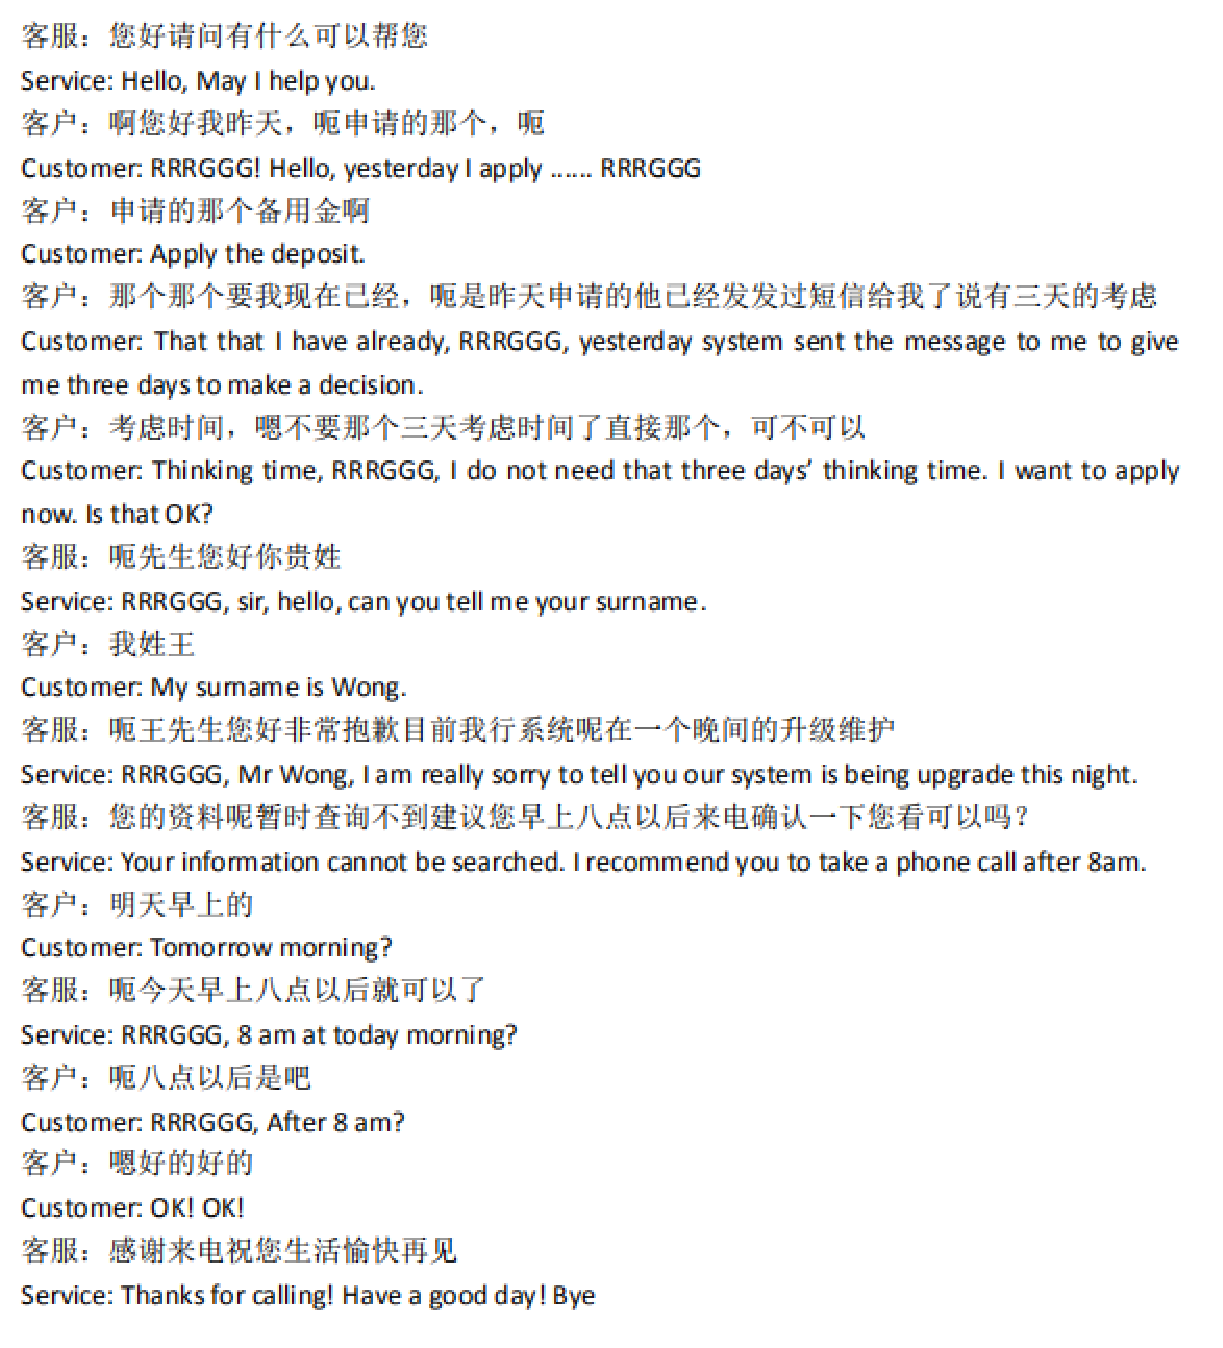
\includegraphics[width=3.6in]{figures/PinganSampleTCS.eps}
\caption{A Sample for Ping An Telephone Customer Service Transcription (The customer information has already been removed.) }
\label{fig:PinganSampleTCS}
\end{figure}

\subsection{Overview}
The proposed system is an ensemble of three modules (See in Figure \ref{fig:PinganSRE},) that are: (i) an ASR module for generating recognized text from input mixed audio. (ii) a Customer/Service identification module for classifying speakers and identify the customer's audio files. Thus, we can get the cleaned one-person single track audio file as input to the SV module. (iii) a speaker verification module, with the input of split audio of customer, verifying the identity of a speaker. The details are shown in the following parts.

\begin{figure*}[htbp]
\centering
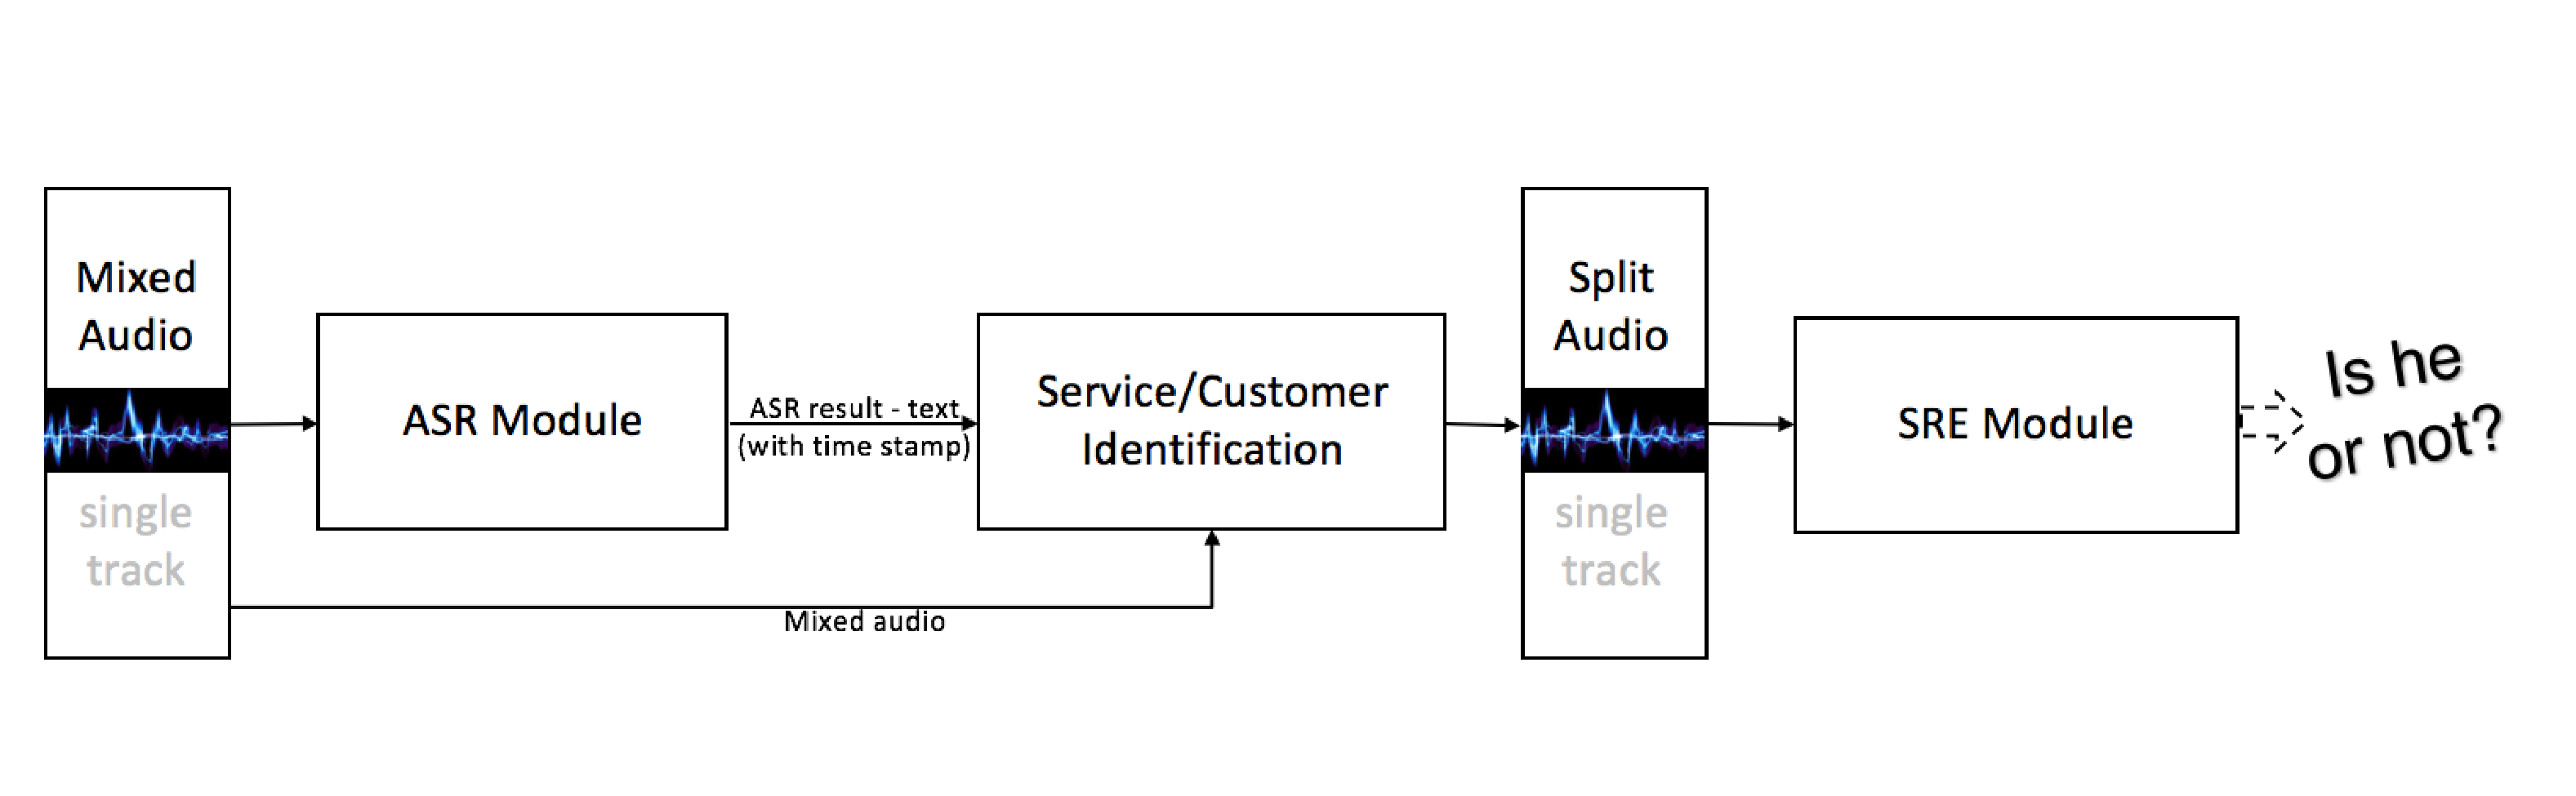
\includegraphics[width=5.4in]{figures/PinganSRE.eps}
\caption{SV Framework for designed Co-Channel TCS}
\label{fig:PinganSRE}
\end{figure*}


\subsection{ASR Module}
\label{sec:asrmodule}

The ASR model helps to transcribe co-channel speech to conversational text. The co-channel audio data is often received as a non-overlapped mono audio file although there are two speakers within the audio file and the audio can be segmented into audio data attributed to separate speakers.

Since we wish to send short text to the Customer/Service Identification module, we first apply Sequential Gaussian Mixture Model based Voice Activity Detection (SGMM-VAD) algorithm, described in \cite{Ying2011Noise}, to split the mixed audio into audio segments. The SGMM-VAD comprises two Gaussian components which respectively describe the speech and non-speech log-power distributions, helps to detect audio parts from noisy speech with high signal noise ratio.

The ASR model is then able to transcribe each audio segments into short text (a short example is shown in \ref{fig:PinganSampleTCS}). Specifically, we use Latency-controlled Bidirectional Highway LSTM RNN model (LC-BHLSTM) \cite{Zhang2016Highway} as the acoustic model of our ASR module, to establish the relationship between the input audio signal and the phonemes or other linguistic units that make up speech.

For ASR model setup, the front-end feature consists of 80-dimension log Mel Filterbank (FBANK) with a frame length of 25ms. 3-dimension pitch feature (including probability of Voicing (POV) features) is appended to create 83-dimension feature vector. The LC-BHLSTM has 5 layers, with 1024 memory cells together with a 512-node projection layer at each layer��s output. The output targets are 10k dimensional context-dependent tied triphone states (a.k.a. senones,) of which were determined by the HMM-GMM training stages.

\subsection{Customer/Service Identification}

The customer/service identification module uses the supervised learning classification approach, to identify the customer and service label from the transcribed text. In the training stage, we manually marked the ``customer" and ``service" label to build the training set. After training, we can use this text classification model to automatically assign the ``customer" and ``service" label to the given text segments.

Different from the traditional text/documents, the texts extracted from telephone customer service are very short (the average text length is only about 8.3.) Figure \ref{fig:PinganSampleTCS} shows the sample of Ping An Telephone Customer Service. Each line is the segment of text, e.g., ``Hello, May I help you?" etc. Therefore, to assign the customer/service label to such short text is a real challenge work.

The motivation of our designed method comes from search engine, where people want to know something, they input some queries (key words) into search engine (e.g., google.com, bing.com) to obtain the related information. Like this procedure, the training short-text has been imported into a search engine; the rest short-texts, as the query, are used to search the relevant texts. The label for the text can be easily voted by the searched texts which has the manually marked label.

Figure \ref{fig:ClassificationTCS} shows the framework of customer/service classification. First, system builds the search engine \cite{brin_page_1998} from these training text (extract Chinese word segmentation, then builds the reserved index on these text, etc.) Second, the new short text, as the query, retrieves the top K related texts from these training texts. Third, system uses k-nearest-neighbor (KNN) \cite{Bishop:2006:PRM:1162264} to vote the label to the input text based on the retrieved results. The short-text's query word can be set the different various weight \cite{Salton1988Term} (e.g., Boolean, TF, TF.IDF.) In the experiment section, we show the accuracy of TF-KNN achieves the better accuracy than the other approaches. Leveraging the well studied information retrieval technique, the proposed approach is extremely scale for the large data and can easily add the new training text by updating the index.

\begin{figure}
\centering
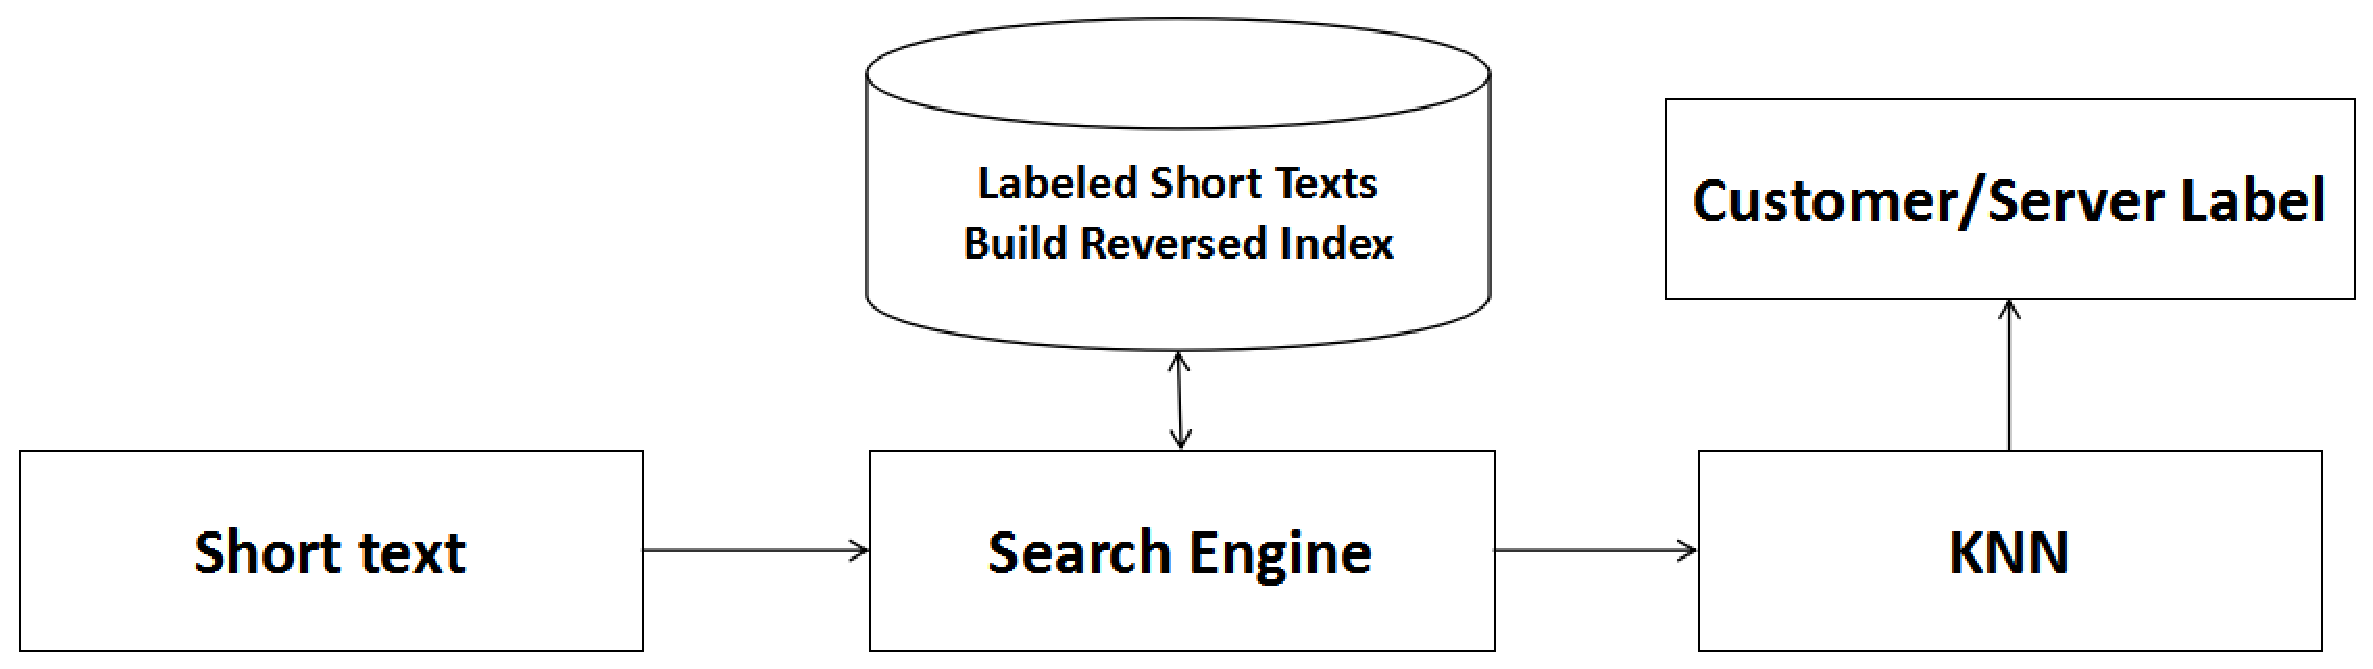
\includegraphics[width=3.4in]{figures/ClassificationTCS.eps}
\caption{Customer/Server Classification for TCS System}
\label{fig:ClassificationTCS}
\end{figure}


\subsection{SV Module}

The framework of many speaker verification applications in use is a GMM-based i-vector system (See Figure \ref{fig:IVectorSV}(a)). It can be decomposed into four sequential stages: the feature extraction, the collection of sufficient statistics, the extraction of i-vectors and a scoring criterion backend. (i) The feature extraction is a process converts the speech waveform into characteristic parameter, which retains useful speaker information from given speech signal and filters unwanted information such as noise. Parameters like Mel-Frequency Cepstrum Coefficient (MFCC,) Linear Predictive Cepstral Coefficient (LPCC) and perceptual linear prediction (PLP) are often used in feature extraction stage, follow by voice activity detection (VAD.) (ii) The collection of sufficient statistics is a process to calculate the zero-order, first-order, second-order Baum-Welch statistics from a sequence of feature vector from the first stage. These statistics are highly dimensional, which is generated from a large GMM, called Universal Background Model (UBM.) (iii) The extraction of i-vectors in the third stage is a technique that converts the high dimensional statistics into a single low dimension feature vector, which carries only the discriminative characteristic information apart from the other speakers. (iv) Once i-vectors are extracted, a scoring criterion backend is used to make decision that whether accept or reject the person as the request identity. There are three commonly used scoring criterions for voice recognition, cosine distance similarity, linear discriminant analysis (LDA) and probabilistic linear discriminant analysis (PLDA.)

\begin{figure}
\begin{minipage}{1.0\linewidth}
  \centerline{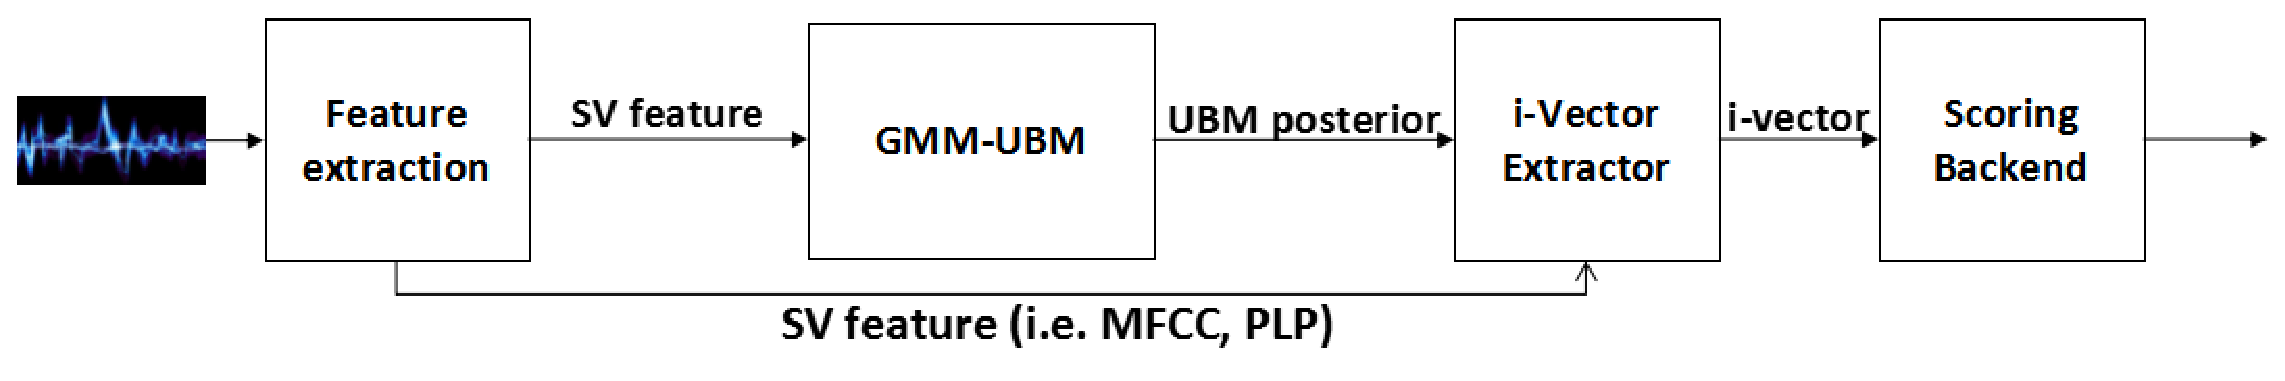
\includegraphics[width=9.0cm]{figures/GMM-UBM.eps}}
  \centerline{ \begin{scriptsize} (a) GMM-UBM \end{scriptsize}}
\end{minipage}
\vfill
\begin{minipage}{1.0\linewidth}
  \centerline{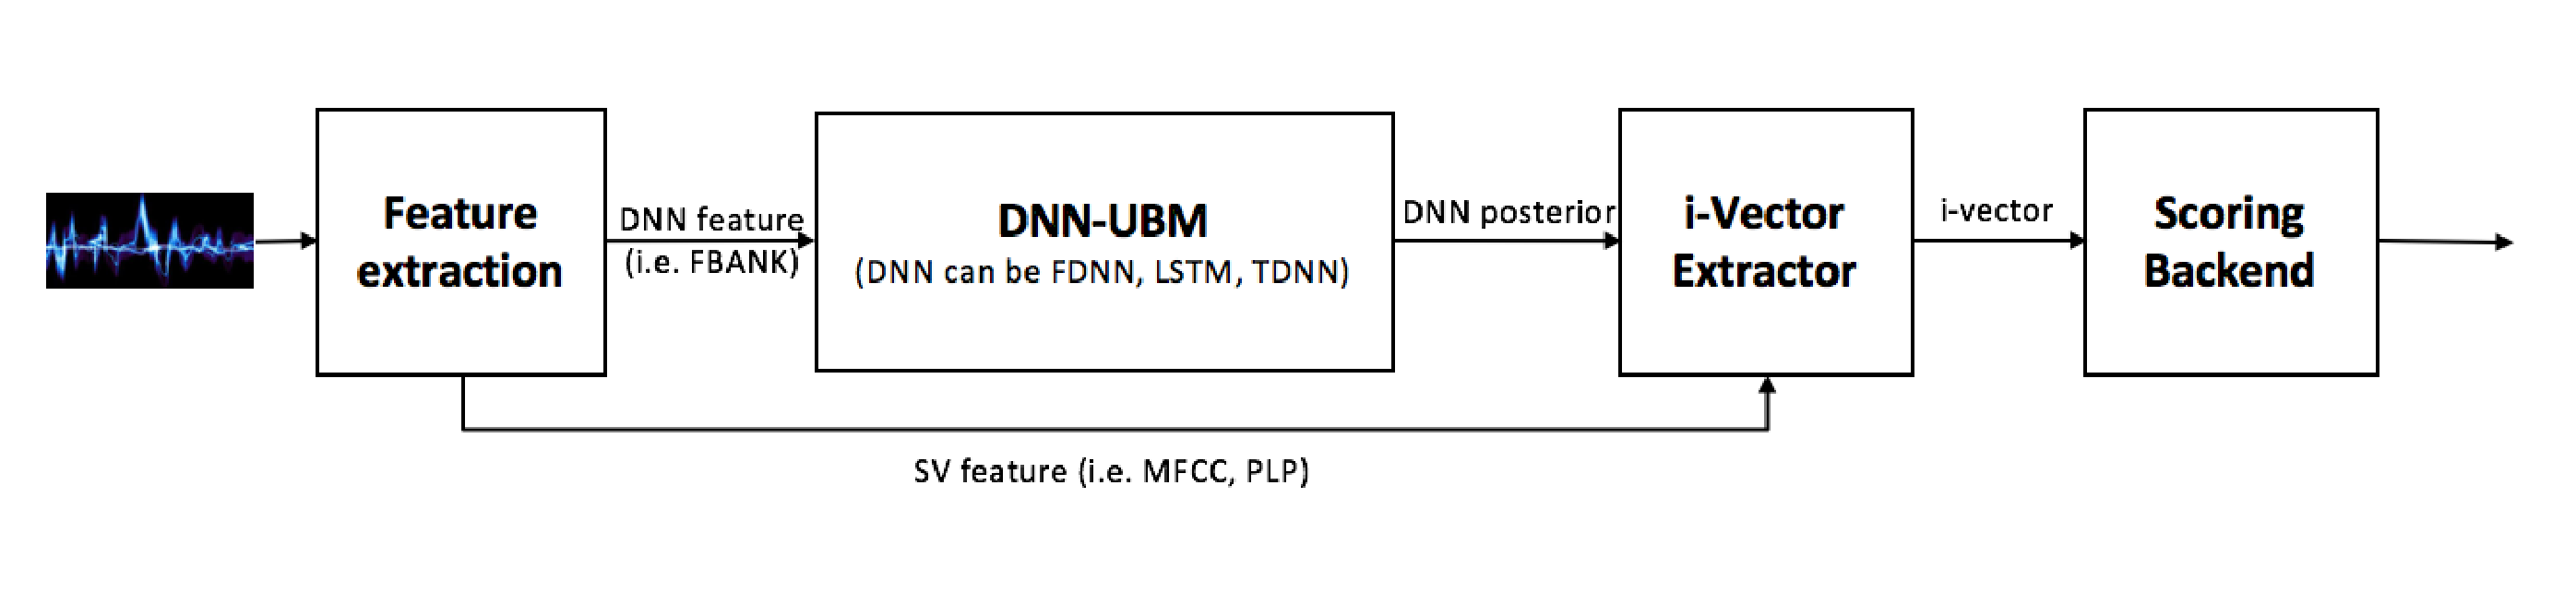
\includegraphics[width=9.0cm]{figures/DNN-UBM.eps} }
  \centerline{ \begin{scriptsize} (b) DNN-UBM \end{scriptsize}}
\end{minipage}
\caption{I-Vector based Speaker Verification Framework}
\label{fig:IVectorSV}
\end{figure}

In the DNN-UBM i-vector framework (See Figure \ref{fig:IVectorSV}(b)), the feature extraction stage stays the same as the GMM-UBM i-vector framework. The different part is that the UBM now utilizes senone states to evaluate the acoustic feature space. In the experiment section, we have tested various kinds of deep neural network to find the best prototype model in our DNN-UBM framework. We show that the Highway LSTM based Universal Background Model (HLSTM-UBM) outperforms the other type of neural network based UBM with comprehensive comparison in accuracy and response time.
